\chapter{Diseño e Implementación} % Main chapter title

\label{Chapter3} % Change X to a consecutive number; for referencing this chapter elsewhere, use \ref{ChapterX}
\definecolor{mygreen}{rgb}{0,0.6,0}
\definecolor{mygray}{rgb}{0.5,0.5,0.5}
\definecolor{mymauve}{rgb}{0.58,0,0.82}

\lstset{ %
  backgroundcolor=\color{white},   % choose the background color; you must add \usepackage{color} or \usepackage{xcolor}
  basicstyle=\footnotesize,        % the size of the fonts that are used for the code
  breakatwhitespace=false,         % sets if automatic breaks should only happen at whitespace
  breaklines=true,                 % sets automatic line breaking
  captionpos=b,                    % sets the caption-position to bottom
  commentstyle=\color{mygreen},    % comment style
  deletekeywords={...},            % if you want to delete keywords from the given language
  %escapeinside={\%*}{*)},          % if you want to add LaTeX within your code
  %extendedchars=true,              % lets you use non-ASCII characters; for 8-bits encodings only, does not work with UTF-8
  %frame=single,	                   % adds a frame around the code
  keepspaces=true,                 % keeps spaces in text, useful for keeping indentation of code (possibly needs columns=flexible)
  keywordstyle=\color{blue},       % keyword style
  language=[ANSI]C,					% the language of the code
  %otherkeywords={*,...},           % if you want to add more keywords to the set
  numbers=left,                    % where to put the line-numbers; possible values are (none, left, right)
  numbersep=5pt,                   % how far the line-numbers are from the code
  numberstyle=\tiny\color{mygray}, % the style that is used for the line-numbers
  rulecolor=\color{black},         % if not set, the frame-color may be changed on line-breaks within not-black text (e.g. comments (green here))
  showspaces=false,                % show spaces everywhere adding particular underscores; it overrides 'showstringspaces'
  showstringspaces=false,          % underline spaces within strings only
  showtabs=false,                  % show tabs within strings adding particular underscores
  stepnumber=1,                    % the step between two line-numbers. If it's 1, each line will be numbered
  stringstyle=\color{mymauve},     % string literal style
  tabsize=2,	                   % sets default tabsize to 2 spaces
  title=\lstname,                   % show the filename of files included with \lstinputlisting; also try caption instead of title
  morecomment=[s]{/*}{*/}%
}


%----------------------------------------------------------------------------------------
%	SECTION 1 : Diseño de Firmware
%----------------------------------------------------------------------------------------
\section{Diseño de Firmware}

\subsection{Punto de partida} 

Al tomar el port de MicroPython para la EDU-CIAA-NXP, era posible ejecutar un intérprete \textit{REPL}\footnote{REPL: Read Eval Print Loop. Mecanismo que toma una expresion escrita por el usuario, la evalua y ejecuta, devolviendo el resultado al usuario.} que provee el proyecto, el cual tiene como standard input (stdin) y standard output (stdout) el puerto serie que la placa tiene conectado a través del conversor USB, de modo que en la PC se crea un COM Virtual que permite a cualquier programa que emula una terminal por puerto serial, conectarse a dicho intérprete.

\begin{figure}[h]
  \centering
    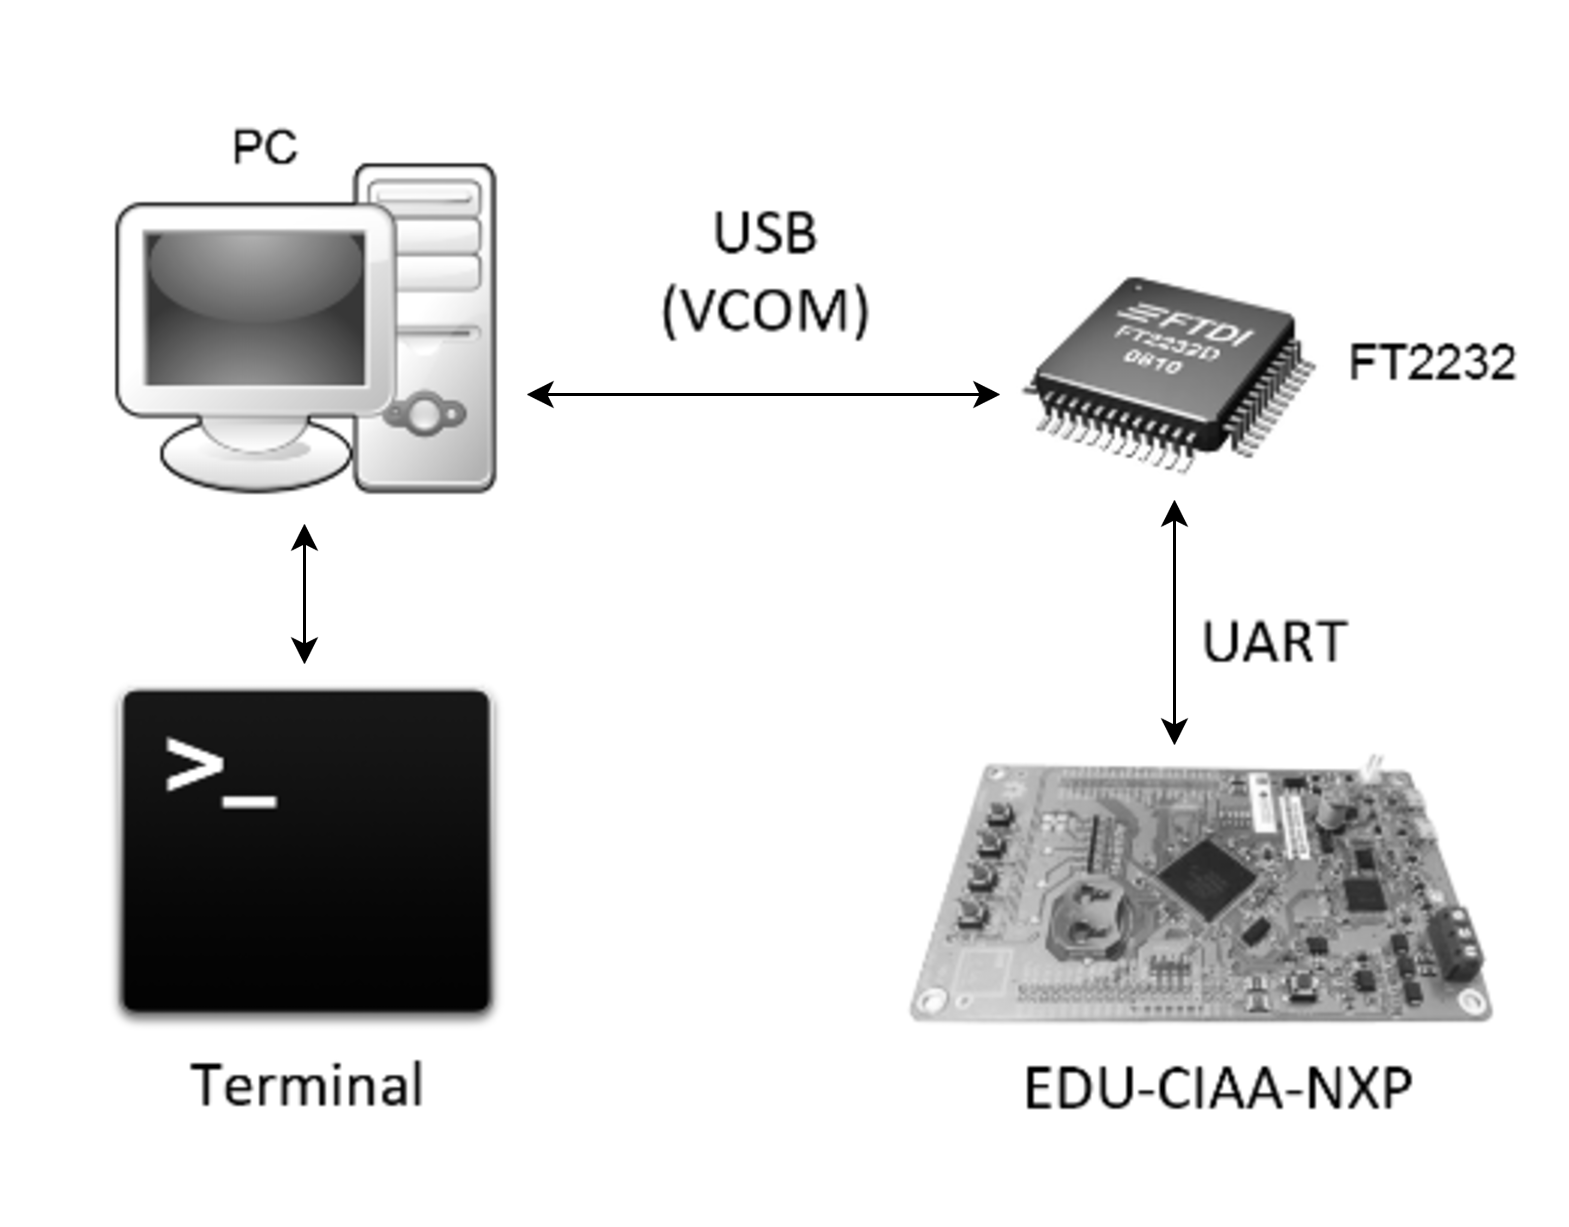
\includegraphics[width=0.7\textwidth]{Figures/fig_conexion}
  \caption{Conexión de la EDU-CIAA-NXP con la PC}
  \label{fig:conexion}
\end{figure}

En la figura \ref{fig:conexion} se observan los bloques que modelan la conexion de la placa con la PC.
Esto permite ejecutar programas que no tengan interacción con el resto del hardware, por ejemplo, se puede escribir:

\begin{verbatim}
>>> print(“Hola mundo”)
\end{verbatim}

Una vez ingresado el codigo, el interprete lo evalua y ejecuta, y el texto "Hola mundo" se transmite por el stdout el cual está ligado a la UART conectada al conversor serie-USB por lo que el texto "Hola mundo" se muestra por la terminal de la PC.

De la misma forma se puede utilizar el sdtin con sentencias como:

\begin{verbatim}
>>> n = input(“Ingrese un numero”)
\end{verbatim}

También se pueden realizar operaciones matemáticas sin inconvenientes:

\begin{verbatim}
>>> a = 27
>>> b = 3
>>> c = a + b
>>> print(c)
\end{verbatim}

Este ultimo ejemplo imprime por la terminal el valor 30.

Pero para interactuar con los periféricos como los pulsadores y los leds, solo existía una versión preliminar de algunas bibliotecas Python creadas previamente por el autor, las cuales se tomaron como punto de partida para el desarrollo profesional de las mismas verificando su correcto funcionamiento por medio de test unitarios y funcionales desarrollados como parte de este trabajo para tal fin.

%----------------------------------------------------------------------------------------

\subsection{Inclusión de bibliotecas Python personalizadas: Módulos y Clases} 

Para poder manejar un periférico, es necesario que al ejecutar una o más funciones de código Python, se ejecute una o más funciones de código C, en la cual se coloca el código necesario para la utilización del periférico en cuestión.

Si bien es posible definir funciones sueltas sin contexto, en Python también es posible la declaración de clases, al ser un lenguaje multiparadigma, el mismo contempla la Programación Orientada a Objetos (POO), mediante la cual se modelaron los periféricos del microcontrolador.

En Python, las clases se agrupan dentro de módulos. Un módulo Python es un conjunto de clases, para poder utilizar una clase que se encuentra dentro de un módulo, deberemos incluir dicho módulo en nuestro programa, mediante la sentencia import, por ejemplo:

\begin{verbatim}
>>> import pyb
\end{verbatim}

El módulo pyb tiene dentro definidas las clases que representan los periféricos del microcontrolador. Una vez incluido el módulo, podremos utilizar las clases definidas dentro de él para crear objetos.
Por ejemplo, para la creación de un objeto que representa el led 1 de la EDU-CIAA-NXP, se escribe:

\begin{verbatim}
>>> import pyb
>>> led = pyb.LED(1)
>>> led.on()
\end{verbatim}

En este ejemplo se utiliza la clase LED para crear el objeto led, la misma recibe como argumento de su constructor, el número de led que el objeto manejará, en este caso, el led 1.

\begin{figure}[ht]
  \centering
    \includegraphics[width=0.8\textwidth]{Figures/fig_calls}
  \caption{Anidamiento de llamadas a funciones desde Python a C}
  \label{fig:calls}
\end{figure}

En la figura \ref{fig:calls} se muestra un diagrama donde se aprecia el \textit{trace}\footnote{Tracing: Log que muestra informacion acerca de la ejecucion de un programa junto con las llamadas a funciones.} de las llamadas a función que se ejecutan cuando el usuario ejecuta desde código Python el método on() de un objeto LED.

En esta figura se observa la llamada del método on() desde el objeto led, esto produce la ejecución de la función pyb\_led\_on() la cual se encuentra definida en el archivo modpybled.c, en este archivo, están declaradas todas las funciones que se mapean a métodos del objeto LED.
Estos archivos modpybXXX.c representan la clase de un periférico (en este ejemplo modpybled.c representa la clase LED) y utilizan las funciones de la capa de abstracción de hardware (uPython HAL) definidas en ciaanxp\_mphal.c para acceder y utilizar los periféricos.
Dentro de la capa uPython HAL, se utilizan las funciones definidas en la capa Board Support Package (archivo board.c) en donde se utilizan las funciones de la biblioteca \textit{LPCOpen}\footnote{LPCOpen: Biblioteca desarrollada por NXP la cual provee macros y funciones para acceder a los registros del microcontrolador desde lenguaje C.} para el manejo de periféricos.

\begin{figure}[ht]
  \centering
    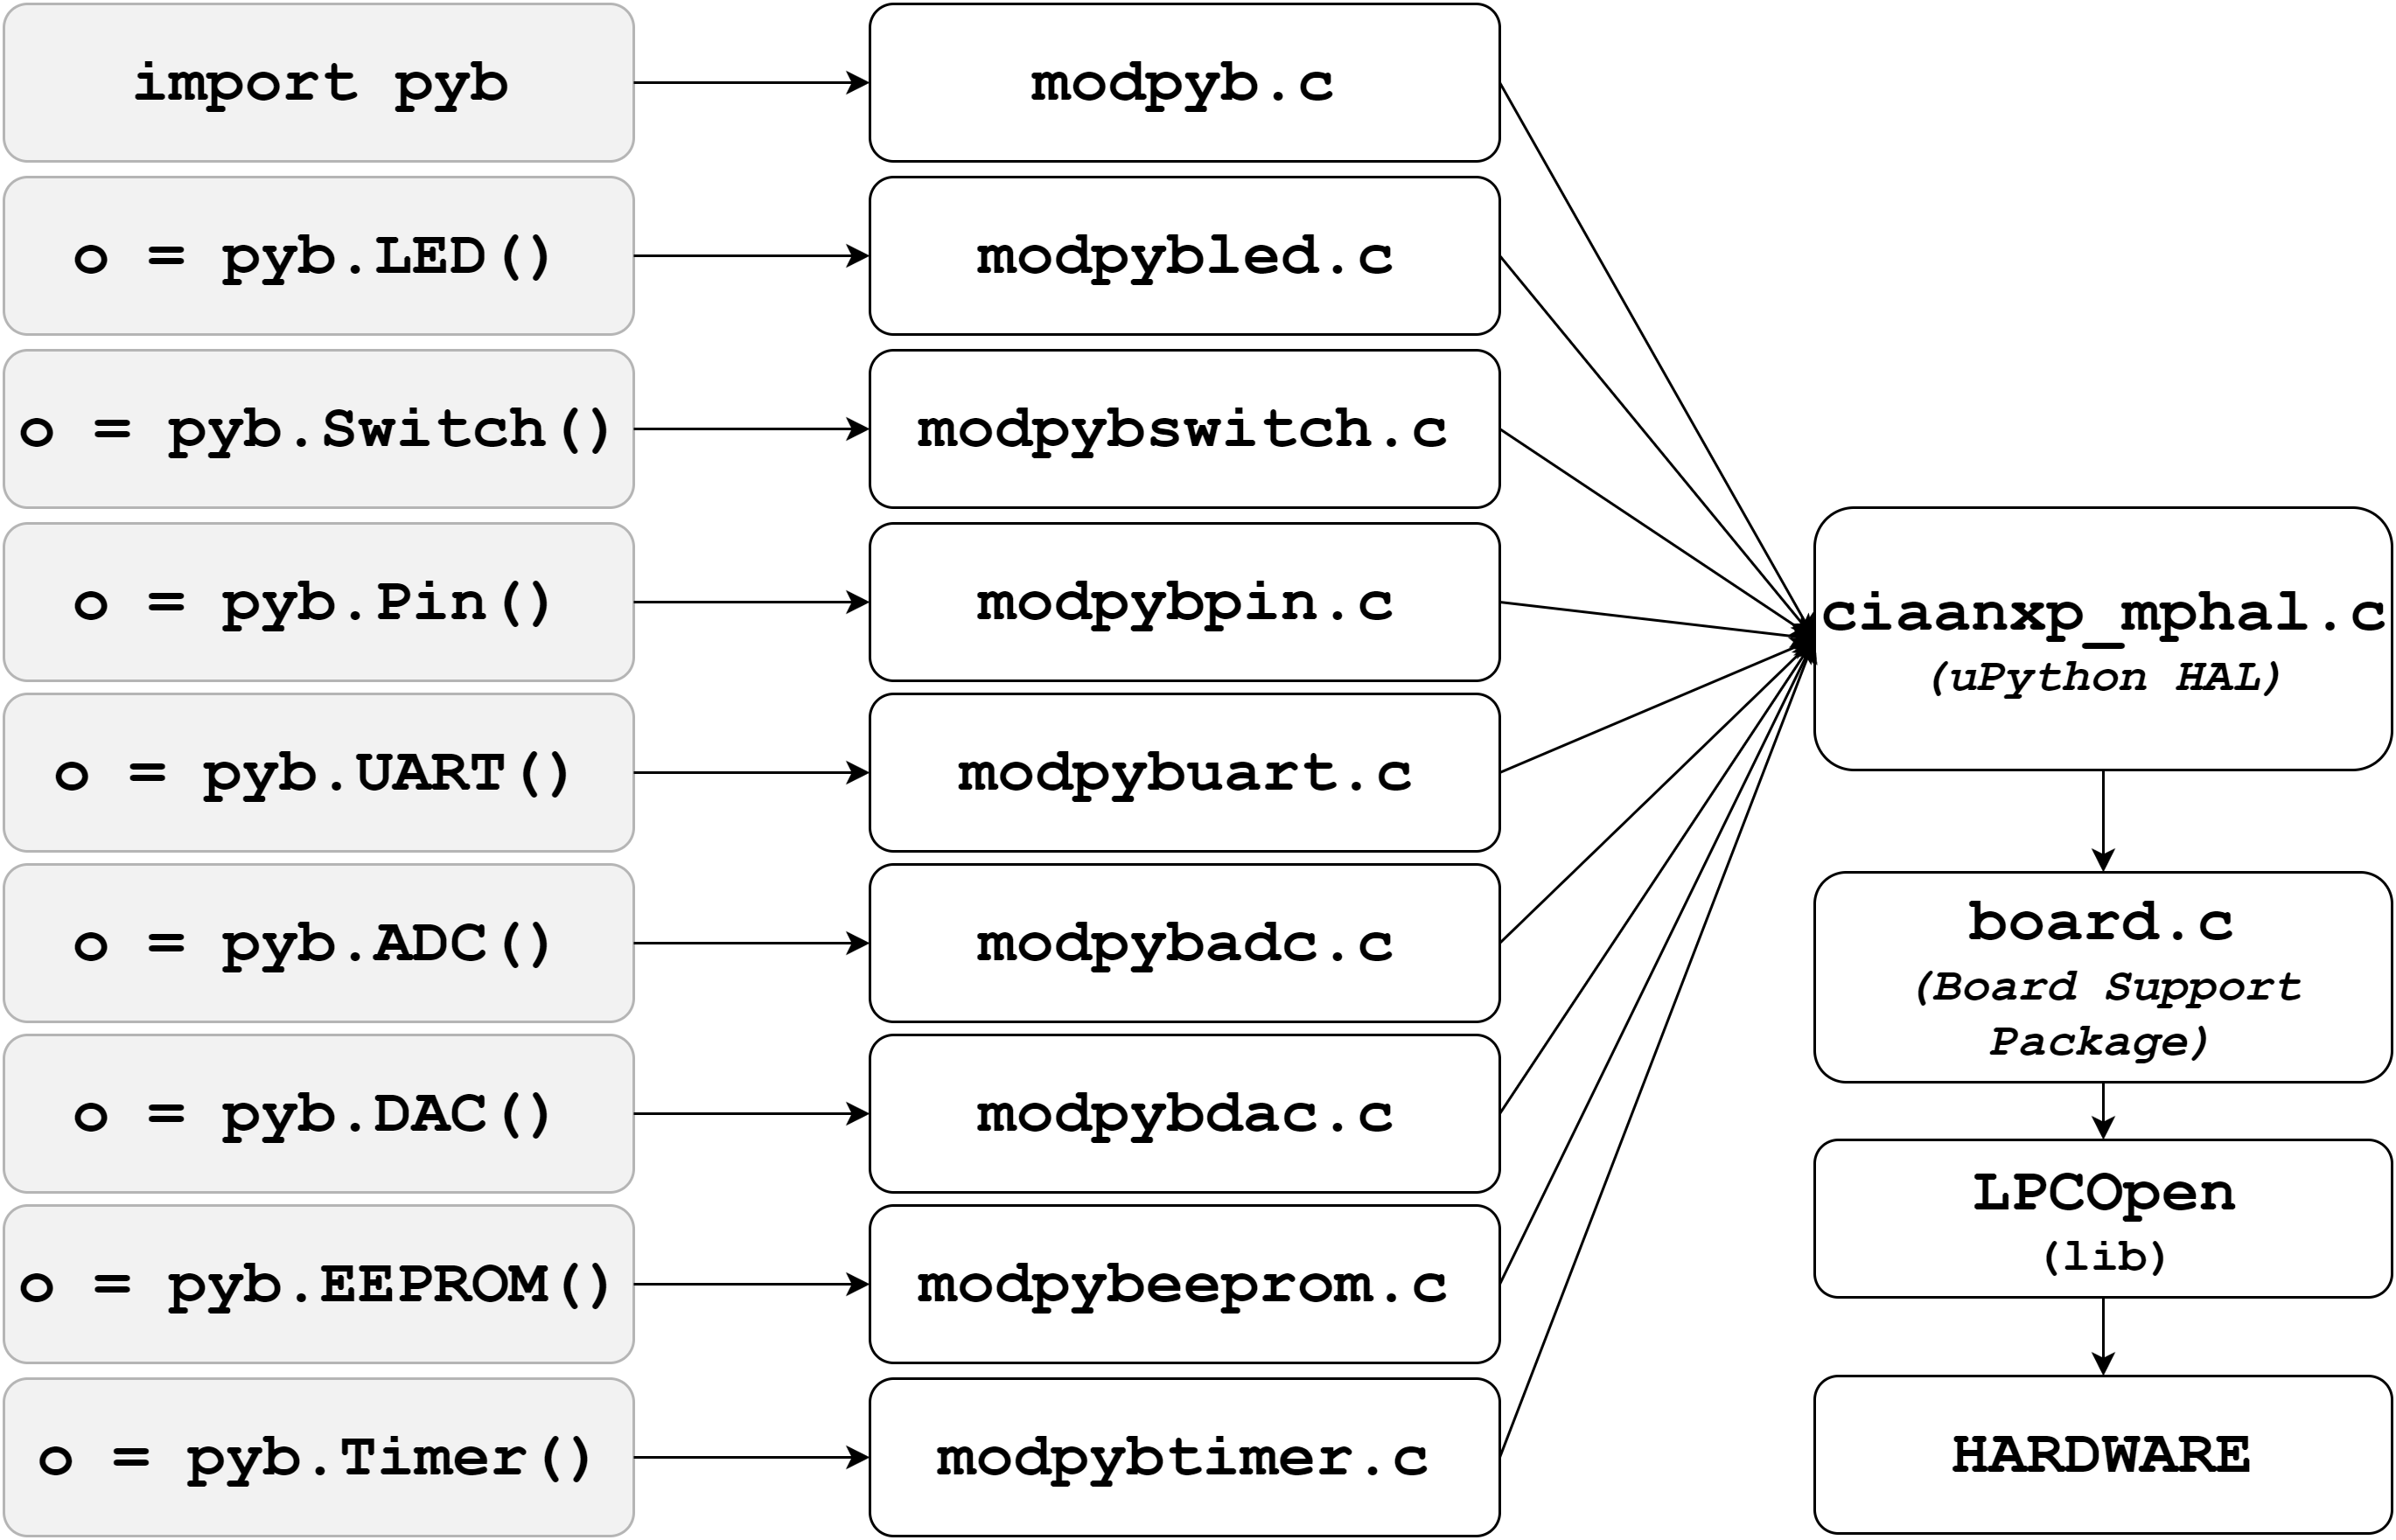
\includegraphics[width=0.9\textwidth]{Figures/fig_files}
  \caption{Relación entre las clases Python y los archivos del Firmware}
  \label{fig:files}
\end{figure}

En la figura \ref{fig:files} se observan los archivos implicados para poder brindar desde el código Python una interfaz para el uso de cada periférico.
Para más detalles sobre el desarrollo de una clase Python desde código C, referirse al ANEXO 1

%----------------------------------------------------------------------------------------

\subsection{Diseño de bibliotecas para el manejo de periféricos desde C}

En el archivo board.c y board.h se definio la capa BSP, mediante la cual se accede a los perifericos del microcontrolador, en este archivo se definieron las funciones para inicializar y utilizar dichos perifericos, requiriendo la menor cantidad de datos de inicializacion posibles y abstrayendo en gran medida la arquitectura del microprocesador.

Esta capa utiliza la biblioteca LPCOpen, la cual es de mas bajo nivel pero permite un facil acceso a los registros del microcontrolador, proveyendo funciones y macros para resolver este problema.

Las funciones definidas en board.c tienen el formato:

\begin{verbatim}
Board_NombrePeriferico_NombreFuncion()
\end{verbatim}

Algunos ejemplos de las funciones que pueden encontrarse en este archivo son:

\begin{verbatim}
void Board_LED_Set(uint8_t LEDNumber, bool On);
bool Board_LED_Test(uint8_t LEDNumber);
void Board_LED_Toggle(uint8_t LEDNumber);
\end{verbatim}

Todos los periféricos tienen su función Init:
\begin{verbatim}
Board_NombrePeriferico_Init()
\end{verbatim}

La cual se encarga de inicializar dicho periférico, existe tambien en el archivo definida una función principal que se encarga de llamar a todas las funciones “Init” y es llamada “Board\_Init()”

Como se indica en la figura \ref{fig:calls}, las funciones definidas en esta capa son ejecutadas por las funciones definidas en la capa Python HAL, las cuales se definen en el archivo ciaanxp\_mphal.c y ciaanxp\_mphal.h.

La capa Python HAL, es practicamente transparente, ya que en la mayoria de los casos no agrega funcionalidades, y simplemente invoca a las funciones de la capa BSP. 
Sin embargo en algunos casos en donde las funciones definidas en BSP no cubren las caracteristicas neecesarias para ser utilziadas desde Python, se han agregado las caracteristicas en esta capa.
Tambien se han agregado porciones de codigo para validacion de rangos, por ejemplo, la funcion para enviar por el puerto serie tiene la forma:

\begin{lstlisting}[caption=Función de envío por la UART de la capa uPython HAL] 
uint32_t mp_hal_rs232_write(uint8_t const * const buffer, 
                                     uint32_t size,uint32_t delay)
{
    if(delay==0)
        return Board_UART_Write(LPC_USART3,buffer,size);

    uint32_t i=0;
    while(size>0)
    {
        Board_UART_Write(LPC_USART3,&(buffer[i]),1);
        mp_hal_milli_delay(delay);
        size--;
        i++;
    }
    return i;
}
\end{lstlisting}

En este caso se observa que la funcion de la capa Python HAL tiene un argumento que indica un delay entre cada byte que se envia, funcionalidad que no existe en la capa BSP, ya que solo se dispone de la funcion “Board\_UART\_Write()” la cual recibe el buffer a transmitir.
En esta funcion se evalua el valor del argumento delay,y en el caso de que sea mayor a cero, se haran envios de 1 byte y luego se ejecutará la función “mp\_hal\_milli\_delay()” la cual boquea el codigo por el tiempo especificado.

Las funciones de la capa Python HAL tienen la forma:

\begin{verbatim}
mp_hal_nombrePeriferico_nombreFuncion()
\end{verbatim}

Tanto la biblioteca board.c como la capa Python HAL puede utiizarse de forma aislada en un proyecto baremetal para el microcontrolador LPC4337, proveyendo un acceso simple a los perifericos del mismo.

%----------------------------------------------------------------------------------------

\subsection{Diseño de bibliotecas para el manejo de periféricos desde Python}

Se pretendió modelar cada periférico mediante una clase, si bien era posible definir funciones pertenecientes al módulo pyb, sin definir clases, por ejemplo:
\begin{verbatim}
>>> pyb.setLed(1,0)
\end{verbatim}

Se decidió respetar el modelo orientado a objetos por las siguientes razones:

\begin{itemize}
	\item El proyecto MicroPython original utiliza este modelo para acceder a los periféricos
	\item Ayuda al entendimiento de programación orientada a objetos (POO), en donde la premisa más básica es representar objetos del mundo real, en este caso un objeto Switch representara un pulsador físico en la placa, generando un ejemplo muy claro del concepto.
	\item Para el uso básico y explicaciones de algoritmo, no es necesario tener los conocimientos de POO, simplemente se trata al objeto como una variable, y no se generan grandes trabas en el momento del aprendizaje.
\end{itemize}

Una vez definido el modelo a utilizar, se optó por mantener, en lo posible, los mismos métodos 

\begin{figure}[ht]
  \centering
    \includegraphics[width=0.99\textwidth]{Figures/fig_classes_diagram}
  \caption{Diagrama de clases para manejo de periféricos}
  \label{fig:classes}
\end{figure}


%----------------------------------------------------------------------------------------
%	SECTION 2: Diseño del Software
%----------------------------------------------------------------------------------------
\section{Diseño del Software}

\subsection{Punto de partida} 

\subsection{Características del IDE} 

\subsection{Diseño del IDE} 

\subsection{Envío del archivo a la placa}

%----------------------------------------------------------------------------------------
%	SECTION 3: Documentacion
%----------------------------------------------------------------------------------------
\section{Documentación}

\subsection{Diseño de proyectos de ejemplo} 

\subsection{Documentación de las bibliotecas implementadas} 



